To reliably laser cool and trap ions into crystals, it is ideal to have ultra-high vacuum (UHV) which is generally defined as having a pressure $<10^{-9}$ Torr. The characteristic collision rate between a monopole and polarizable neutral is defined by the $C_4/r^4$ attractive term and is called the Langevin collision rate. In a vacuum chamber, we tend to find the predominant gas left after baking is \ce{H2}, which will have collisions with the trapped ions at the Langevin rate.

By knowing the rate of

\begin{equation}
	\ce{Be+(^2P3/2) + H2 -> BeH+ + H}
	\label{eq: Be+H2->BeH}
\end{equation}

to be \todo{rate}\cite{Roth2006}. With an ion gauge, we find our vacuum to be $\approx 1 \times 10^{-10}$ Torr, and verified via \ce{Be+} fluorescence decay due to reactions with background \ce{H2}.

We want to make sure that there is as little \ce{H2O} in the chamber as possible to ensure that the data we take with the water from the CBGB is exclusively from the CBGB and not due to background water collisions.

\begin{figure}[H]
	\centering
	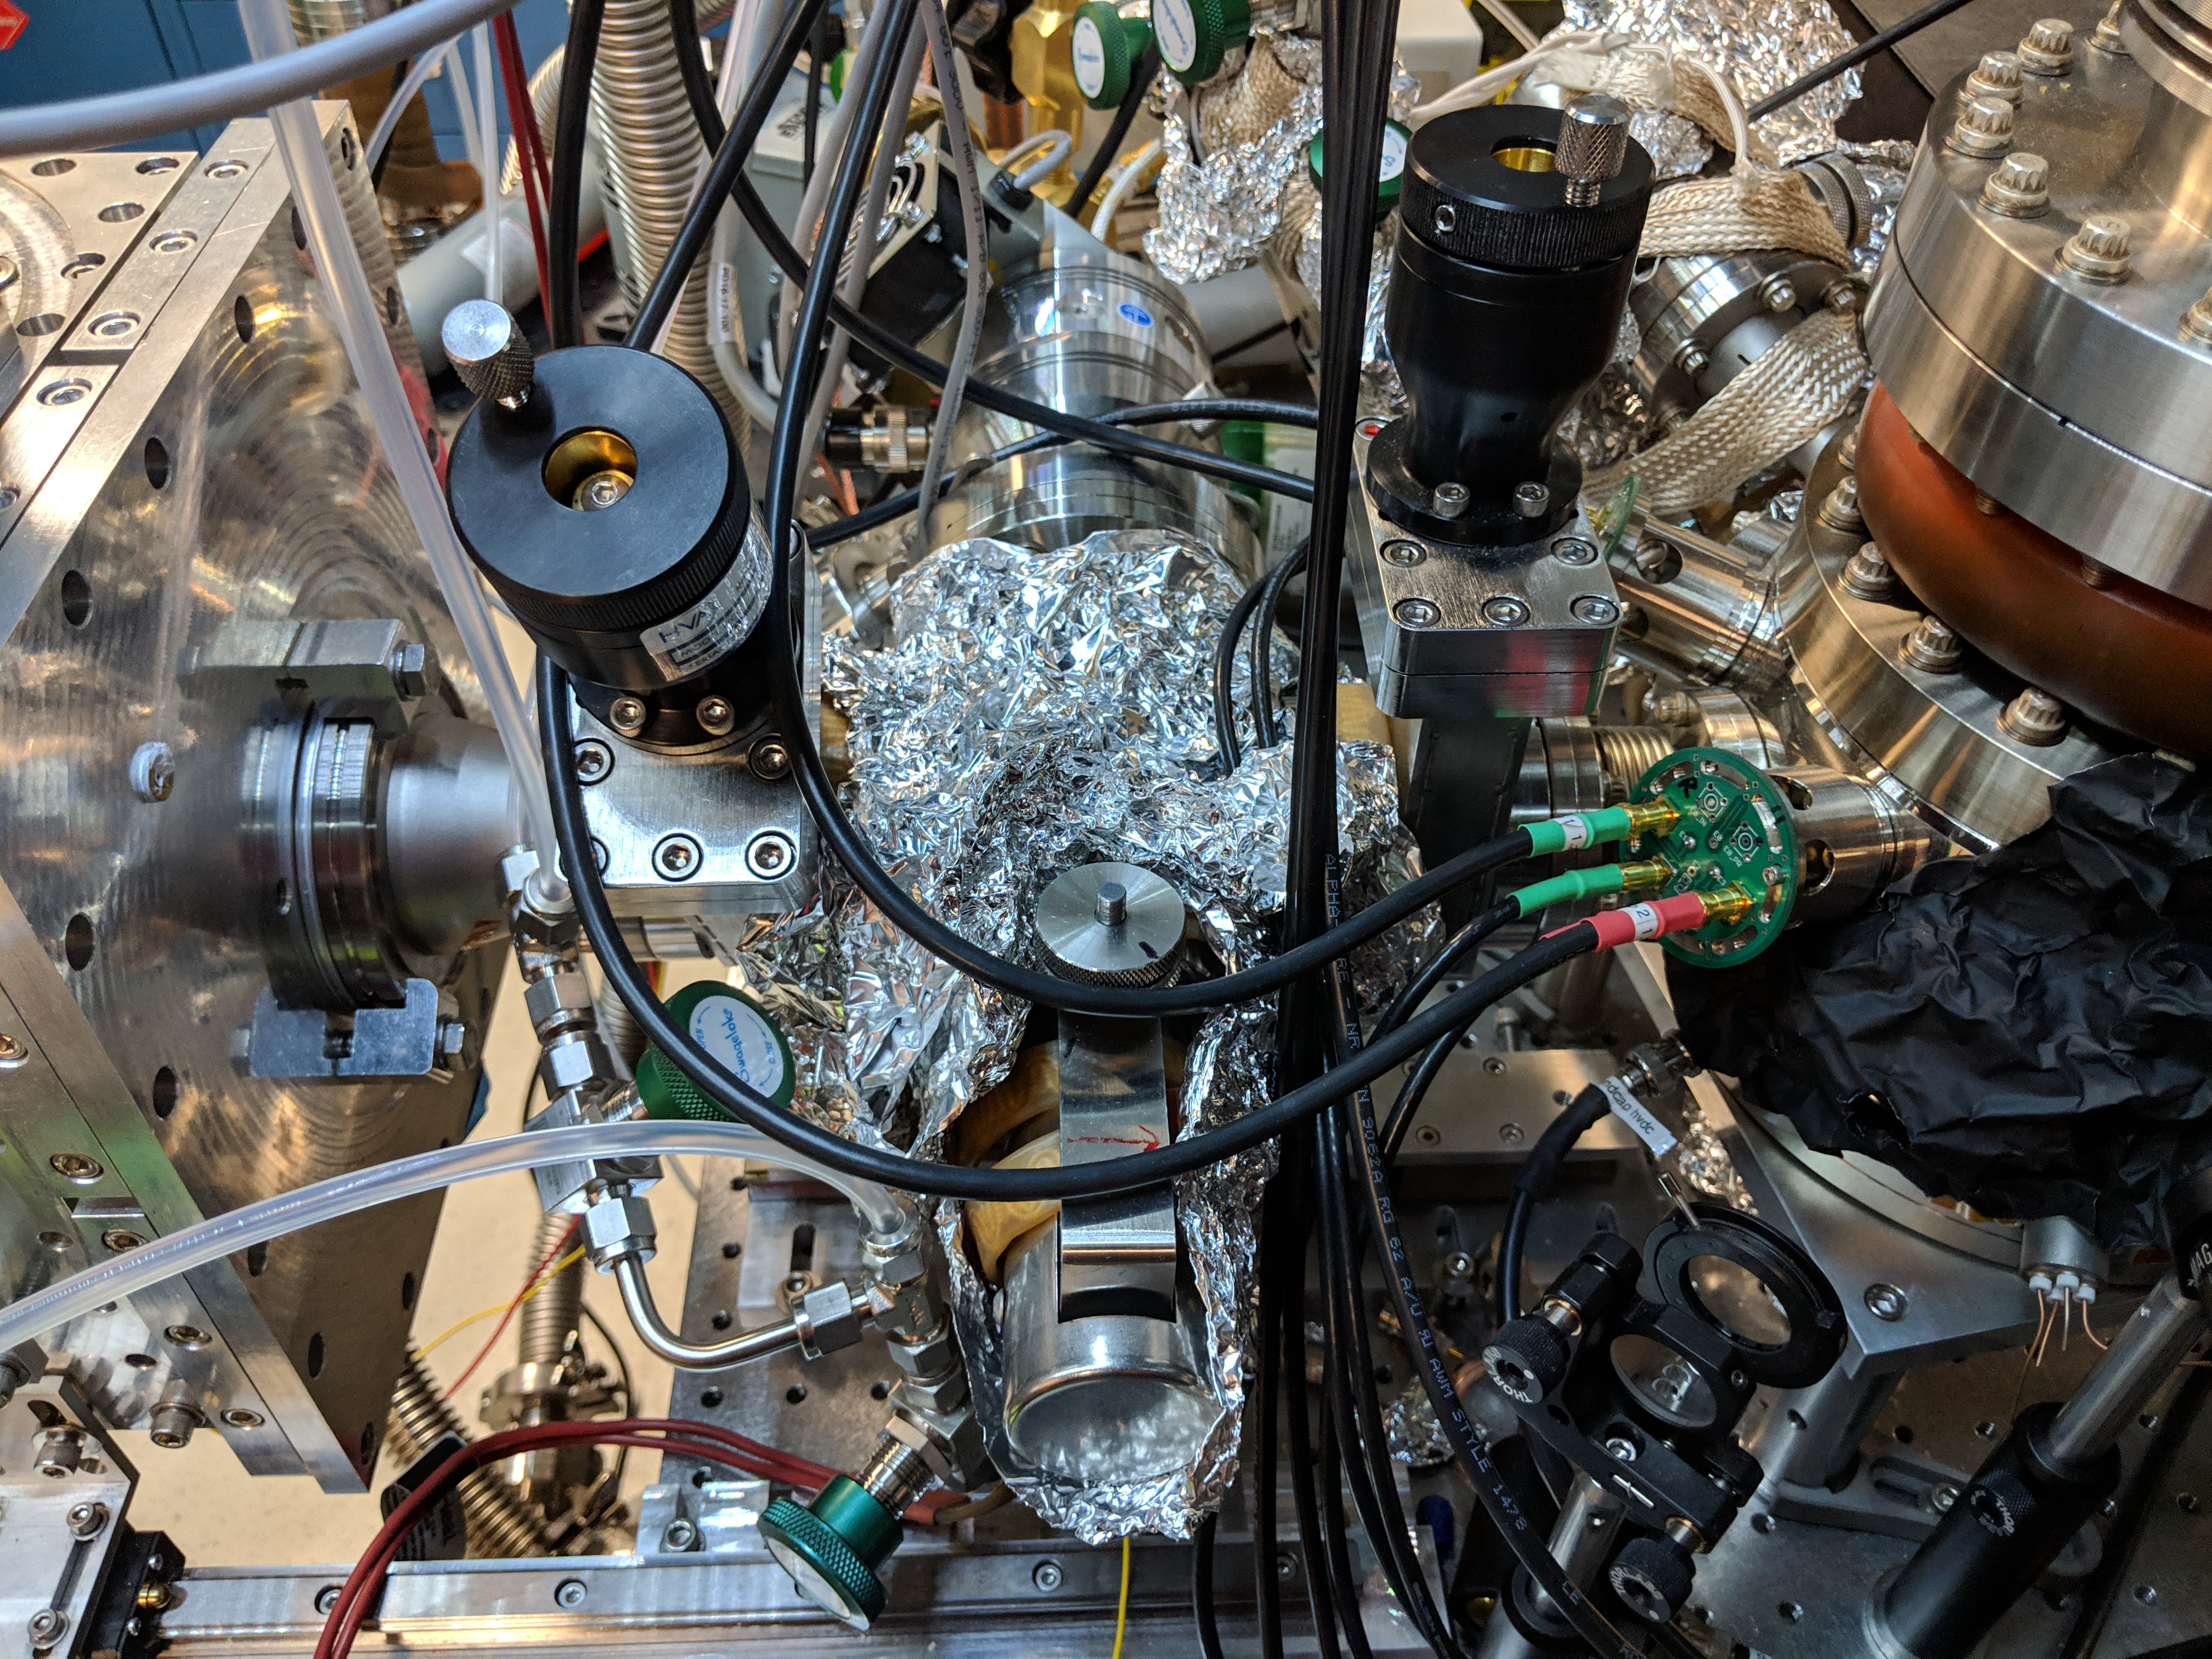
\includegraphics[width=0.8\textwidth]{images/differential_pumping.jpg}
	\caption{Differential pumping region in between the stem and ion trap chambers with gate valves on either end. Blank copper CF gaskets with apertures of 4 mm and 10 mm are placed towards the stem and ion chamber respectively to limit conductance of background gasses while allowing the cryogenic beam through. An Agilent Twistorr 84 FS turbo pump keeps the region at pressures around $10^{-10}$ Torr and a leak valve allows for controlled introduction of secondary gasses.}
\end{figure}